\documentclass{article}
\usepackage[utf8]{inputenc}
\usepackage{t1enc}
\usepackage{geometry}
 \geometry{
 a4paper,
 total={210mm,297mm},
 left=20mm,
 right=20mm,
 top=20mm,
 bottom=20mm,
 }
\usepackage{amsmath}
\usepackage{amssymb}
\frenchspacing
\usepackage{fancyhdr}
\pagestyle{fancy}
\lhead{Urbán János tanár úr feladatsorai}
\chead{C08/08/1.}
\rhead{Gráfok}
\lfoot{}
\cfoot{\thepage}
\rfoot{}

\usepackage{pgf,tikz}
\usetikzlibrary{arrows,trees}

\usepackage{array}

\usepackage{enumitem}
\usepackage{multicol}
\usepackage{calc}
\newenvironment{abc}{\begin{enumerate}[label=\textit{\alph*})]}{\end{enumerate}}
\newenvironment{abc2}{\begin{enumerate}[label=\textit{\alph*})]\begin{multicols}{2}}{\end{multicols}\end{enumerate}}
\newenvironment{abc3}{\begin{enumerate}[label=\textit{\alph*})]\begin{multicols}{3}}{\end{multicols}\end{enumerate}}
\newenvironment{abc4}{\begin{enumerate}[label=\textit{\alph*})]\begin{multicols}{4}}{\end{multicols}\end{enumerate}}
\newenvironment{abcn}[1]{\begin{enumerate}[label=\textit{\alph*})]\begin{multicols}{#1}}{\end{multicols}\end{enumerate}}
\setlist[enumerate,1]{listparindent=\labelwidth+\labelsep}

\newcommand{\degre}{\ensuremath{^\circ}}
\newcommand{\tg}{\mathop{\mathrm{tg}}\nolimits}
\newcommand{\ctg}{\mathop{\mathrm{ctg}}\nolimits}
\newcommand{\arc}{\mathop{\mathrm{arc}}\nolimits}
\renewcommand{\arcsin}{\arc\sin}
\renewcommand{\arccos}{\arc\cos}
\newcommand{\arctg}{\arc\tg}
\newcommand{\arcctg}{\arc\ctg}

\parskip 8pt
\begin{document}

\section*{Gráfok}

\subsection*{2010. 04. 29.}
\begin{enumerate}
\item Be lehet-e járni egy a.) kocka b.) oktaéder csúcsait egy csúcsból indulva, az élek mentén haladva úgy, hogy minden csúcsot pontosan egyszer érintsünk és a végén visszaérjünk a kiindulási csúcsba?
\item Szervezzünk 8 csapat körmérkőzéses versenyéhez első három fordulót, ha az egyes fordulók mérkőzőseit egy időben kell lejátszani. Ábrázoljuk a tervezetet gráffal.
\item 8 csapat körmérkőzéses versenye során előfordulhat-e, hogy az egyes csapatok eddig rendre $1; 2; 2; 2; 4; 5; 7; 7;$ mérkőzést játszottak?
\item Igazoljuk, hogy ha $n$ csapat ($n\geq 4$, egész) körmérkőzéses versenyén (legalább) $n+1$ mérkőzést már lejátszottak, akkor van olyan csapat, amelyik már legalább háromszor játszott.
\item Hány olyan 5 csúcsú egyszerű gráf van, melyben a csúcsok fokszáma 1, 2, 2, 3?
\item Egy 6 csúcsú egyszerű gráf csúcsainak fokszáma 2, 2, 3, 3, 5, 5. hány ilyen gráf van? Hány éle van a gráfnak?
\end{enumerate}


\subsection*{2010. 05. 05.}
\begin{enumerate}
\item Egy 5 csúcsú egyszerű gráfnak 8 éle van. Mekkorák lehetnek a csúcsok fokszámai?
\item Hány csúcsú az a \underline{teljes} \underline{egyszerű} gráf, amelynek kevesebb éle van, mint a csúcsok számának 6-szorosa, de több, mint a csúcsok számának 5-szöröse?
\item Bizonyítsuk be, hogy ha egy $n$ csúcsú ($n>2$, egész) egyszerű gráfban a 0 kivételével minden lehetséges fokszám előfordul, akkor a gráfban két $\frac{n}{2}$ fokú csúcs van.
\item Hány 6 csúcsú, legalább 12 élű egyszerű gráf van?
\item Rajzoljunk két 5 csúcsú egyszerű gráfot, amelyekben a csúcsok fokszámai 1; 2; 2; 2; 3, de a két gráf nem izomorf.
\item Izomorf-e bármely két olyan 8 csúcsú gráf, amelynek minden csúcsa harmadfokú?
\item Igazoljuk, hogy az $n$ csúcsú $C_1$ egyszerű gráf nem tartalmaz zárt töröttvonalat, akkor $C_1$ komplementerének legalább $\frac{(n-1)\cdot(n-2)}{2}$ éle van.
\end{enumerate}


\subsection*{2010. 05. 27.}
\begin{enumerate}
\item Bizonyítsuk be, hogy ha egy gráf minden csúcsának fokszáma legalább 2, akkor van benne kör.
\item Igazoljuk, hogy ha egy $n$ csúcsú gráfnak legalább $n$ éle van, akkor van benne kör.
\item ($*$) Igazoljuk, hogy ha egy egyszerű gráf minden pontjának fokszáma legalább 3, akkor van benne páros hosszúságú kör.
\item Adjunk meg olyan 6 csúcsú egyszerű gráfot, amely nem összefüggő, és minden csúcsa másodfokú.
\item Igazoljuk, hogy egy $n$ szögpontú ($n\geq 1$ egész) összefüggő gráfnak legalább $n-1$ éle van.
\item Rajzoljunk 7 csúcsú, 15 élű nem összefüggő egyszerű gráfot.
\item Igazoljuk, hogy bármely egyszerű gráfban igaz, hogy vagy maga a gráf, vagy a komplementere összefüggő.
\end{enumerate}


\subsection*{2010. 06. 01.}
\begin{enumerate}
\item Hány olyan a.) 8 csúcsú, b.) 9 csúcsú nem összefüggő gráf van, amelynek minden csúcsa legalább harmadfokú?
\item Igazoljuk, hogy ha $\geq 4$ egész, akkor van olyan n csúcsú összefüggő gráf, amelynek komplementere is összefüggő.
\item Igazoljuk, hogy bármely legalább 2 csúcsú fagráfnak van elsőfokú csúcsa. Igaz-e, hogy 2 elsőfokú csúcsa is van egyszerre?
\item Hány különböző 5 csúcsú fa van, ha a csúcsokat nem különböztetjük meg?
\item Igazoljuk, hogy az $n$ csúcsú, $n$ élű egyszerű összefüggő gráfban ($n\geq 3$, egész) biztosan 1 kör van.
\item Hány olyan 8 csúcsú egyszerű gráf van, amelynek minden csúcsa másodfokú (a csúcsokat nem különböztetjük meg)?
\end{enumerate}

\subsection*{2010. 06. 02.}
\begin{enumerate}
\item Igazoljuk, hogy bármely összefüggő gráfnak van olyan részgráfja, amely fa és a gráf  minden csúcsát tartalmazza (a gráf \underline{faváza}).
\item  Egy ,,erdő'' 5 fájában összesen 16 él van. Hány csúcsa van az erdőnek?
\item Hány különböző 5 csúcsú fa van (a csúcsokat nem különböztetjük meg)?
\item Legalább hány élük van az $n$ csúcsú, $k$ komponensű gráfoknak ($n>k>0$, egészek)?
\item Rajzoljuk meg az a.) 6 és b.) 7 csúcsú összefüggő gráfokat, amelyekben nincs kör.
\item Hány olyan 8 csúcsú egyszerű gráf van, amelyben minden csúcs másodfokú (a csúcsokat nem különböztetjük meg)?
\end{enumerate}

\subsection*{2010. 06. 03.}
\begin{enumerate}
\item Van-e olyan egyszerű gráf, amelyben a pontok fokszáma:
\begin{abcn}{2}
\item $ 3, 3, 3, 3, 4, 4, 4, 5$;
\item $ 3, 3, 3, 3, 3, 3, 3, 5$?
\end{abcn}
\item Egy egyszerű gráfban minden pont foka 3. Hány csúcsa (pontja) lehet egy ilyen gráfnak?
\item Adjunk meg 7 csúcsú, legalább 18 élű egyszerű gráfokat.
\item Adjunk meg két 5 csúcsú egyszerű gráfot, amelyben az egyes csúcsok fokszáma 1, 2, 2, 2, 3 és a két gráf nem izomorf.
\item Egy $n$ csúcsú teljes egyszerű gráfnak hány 3 élű, izolált pontot nem tartalmazó részgráfja van ($n\geq 3$)?
\item Rajzoljuk meg a 7 csúcsú összefüggő kör mentes gráfokat.
\end{enumerate}

\newpage

\subsection*{7 csúcsú fák (11 db)}
\begin{center}

\begin{tabular}{m{8cm}m{8cm}}
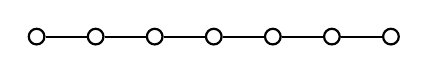
\begin{tikzpicture}[style=thick,scale=0.5] 
\tikzstyle{every node}=[circle,inner sep=2pt,draw] 
\node{\null}[grow'=right] 
child{node{\null} 
child{node{\null} 
child{node{\null}
child{node{\null}
child{node{\null}
child{node{\null}}}}}}};
\end{tikzpicture} 
&
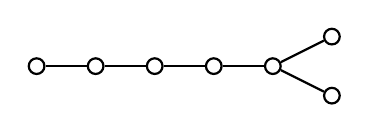
\begin{tikzpicture}[style=thick,scale=0.5] 
\tikzstyle{every node}=[circle,inner sep=2pt,draw] 
\node{\null}[grow'=right] 
child{node{\null} 
child{node{\null} 
child{node{\null}
child{node{\null}
child{node{\null}}
child{node{\null}}}}}};
\end{tikzpicture} 
\cr & \cr & \cr
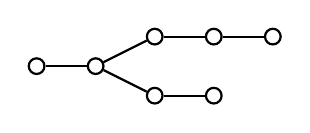
\begin{tikzpicture}[style=thick,scale=0.5] 
\tikzstyle{every node}=[circle,inner sep=2pt,draw] 
\node{\null}[grow'=right] 
child{node{\null} 
child{node{\null} 
child{node{\null}
child{node{\null}}}}
child{node{\null}
child{node{\null}}}};
\end{tikzpicture} 
&
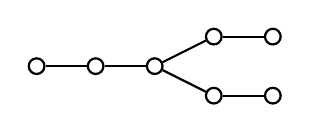
\begin{tikzpicture}[style=thick,scale=0.5] 
\tikzstyle{every node}=[circle,inner sep=2pt,draw] 
\node{\null}[grow'=right] 
child{node{\null} 
child{node{\null} 
child{node{\null}
child{node{\null}}}
child{node{\null}
child{node{\null}}}}};
\end{tikzpicture} 
\cr & \cr & \cr
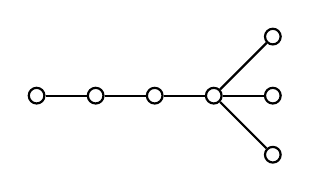
\begin{tikzpicture}[style=thick,scale=0.5] 
\tikzstyle{every node}=[circle,inner sep=2pt,draw] 
\node{\null}[grow'=right] 
child{node{\null} 
child{node{\null} 
child{node{\null}
child{node{\null}}
child{node{\null}}
child{node{\null}}}}};
\end{tikzpicture} 
&
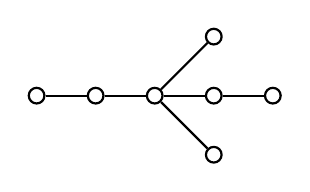
\begin{tikzpicture}[style=thick,scale=0.5] 
\tikzstyle{every node}=[circle,inner sep=2pt,draw] 
\node{\null}[grow'=right] 
child{node{\null} 
child{node{\null} 
child{node{\null}}
child{node{\null}
child{node{\null}}}
child{node{\null}}}};
\end{tikzpicture}
\cr & \cr & \cr
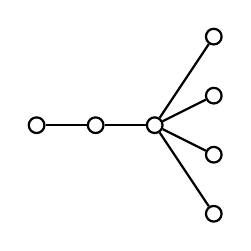
\begin{tikzpicture}[style=thick,scale=0.5] 
\tikzstyle{every node}=[circle,inner sep=2pt,draw] 
\node{\null}[grow'=right] 
child{node{\null} 
child{node{\null} 
child{node{\null}}
child{node{\null}}
child{node{\null}}
child{node{\null}}}};
\end{tikzpicture}
 &
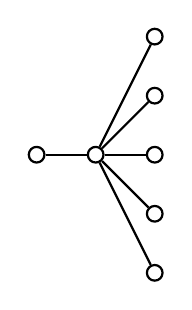
\begin{tikzpicture}[style=thick,scale=0.5] 
\tikzstyle{every node}=[circle,inner sep=2pt,draw] 
\node{\null}[grow'=right] 
child{node{\null} 
child{node{\null}} 
child{node{\null}}
child{node{\null}}
child{node{\null}}
child{node{\null}}};
\end{tikzpicture}
\cr & \cr & \cr
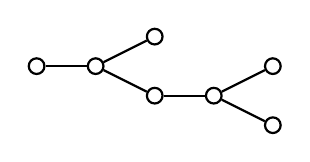
\begin{tikzpicture}[style=thick,scale=0.5] 
\tikzstyle{every node}=[circle,inner sep=2pt,draw] 
\node{\null}[grow'=right] 
child{node{\null} 
child{node{\null}} 
child{node{\null}
child{node{\null}
child{node{\null}}
child{node{\null}}}}};
\end{tikzpicture}
&
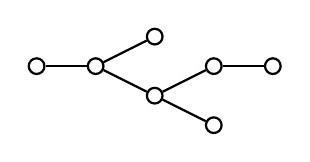
\begin{tikzpicture}[style=thick,scale=0.5] 
\tikzstyle{every node}=[circle,inner sep=2pt,draw] 
\node{\null}[grow'=right] 
child{node{\null} 
child{node{\null}} 
child{node{\null}
child{node{\null}
child{node{\null}}}
child{node{\null}}}};
\end{tikzpicture}
\cr & \cr & \cr
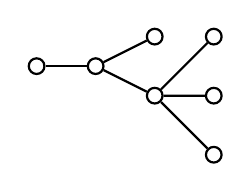
\begin{tikzpicture}[style=thick,scale=0.5] 
\tikzstyle{every node}=[circle,inner sep=2pt,draw] 
\node{\null}[grow'=right] 
child{node{\null} 
child{node{\null}} 
child{node{\null}
child{node{\null}}
child{node{\null}}
child{node{\null}}}};
\end{tikzpicture}
& 
\end{tabular}
\end{center}

\end{document}